\thispagestyle{empty}

%\section*{}%
%\phantomsection%
%\addcontentsline{toc}{section}{\protect\numberline{}Lettre de publication}%
\invisibleunnumberedchapter{Lettre de publication}%

\noindent
\includegraphics[height=3.5cm]{Logo3rd.png} \hfill \hfill 
\includegraphics[height=3cm]{319th.png}%

\vfil

\begin{flushright}Le \today{} à \currenttime{}\end{flushright}%

\vfil%

\vfil%

% \begin{minipage}[c][\textheight][s]{\linewidth}
% \baselineskip=1\baselineskip plus 1fill % stretch as much as needed
% \lineskip=0pt plus 1fill % just for safety
% \docname{} est publié par l'État Major (EM) du \rgt{}.%

%\begin{mini}

Ce document est publié par et pour le \rgt{}.

\vfil%

Le \rgt{} est un escadron évoluant sur le simulateur de combat \dcs{} (DCS), édité par ``Eagle Dynamics'' (ED), membre de l'escadrille virtuelle francophone \thirdwing{}.

\vfil%

Ce document n'engage aucune partie autre que le \rgt{}.

\vfil%

Ce document peut être transmis à tous les membres de la \thirdwing{} sans autorisation préalable, ou à d'autres personnes membres d'un escadron évoluant sur DCS.

\vfil%

Un membre de l'EM du \rgt{} doit être averti lorsque ce document est transmis à un membre d'un autre escadron évoluant sous DCS.

\vfil%

Les commentaires ou suggestions à propos de ce document peuvent être envoyés à: \href{mailto:etcher3rd@gmail.com}{etcher3rd@gmail.com}.

\vfil%

%\end{mini}

\begin{flushright}
    \hfill \parbox{0.3\textwidth}{\raggedright \hfill 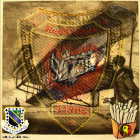
\includegraphics[width=0.1\textwidth]{avatar.png}} \hfil \parbox{0.4\textwidth}{\raggedright etcher \\ Cpt, 319th Rgt \\ \inmem{}}%

\hfill \parbox{0.3\textwidth}{\raggedright \hfill } \hfil \parbox{0.4\textwidth}%
{\centering \includegraphics[width=0.37\textwidth]{signature.png}}%   
\end{flushright}%

\vfil%
%\end{imini}
% \end{minipage}
%\end{onepage}